\documentclass[17pt,a4paper,landscape]{extarticle}
\usepackage[margin=2.35cm,top=0.12cm,left=1.05cm]{geometry}
\usepackage{amsmath}
\usepackage{amssymb}
\usepackage{tasks}
\usepackage{tikz}
\usepackage{xcolor}
\usepackage[sfdefault,lf]{FiraSans}
\renewcommand{\familydefault}{\sfdefault}
\setlength{\parindent}{0pt}
\pagestyle{empty}
\settasks{label=\textbf{\arabic*.}, label-width=2.2em, item-indent=2.95em, column-sep=2.1cm, after-item-skip=4.7em}
\renewcommand{\arraystretch}{1.15}
\everymath{\displaystyle}

\begin{document}
\sffamily
\boldmath

\boldmath

{\LARGE \textbf{Area of basic shapes --- Excellence}}
\begin{tasks}(3)
\task Find the area.\\[0.4em]
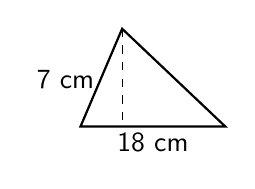
\begin{tikzpicture}[x=0.23cm,y=0.23cm,baseline=(current bounding box.center)]
  \coordinate (A) at (0,0);
  \coordinate (B) at (8,0);
  \coordinate (C) at (2.3,5.4);
  \draw[thick] (A)--(B)--(C)--cycle;
  \draw[dashed] (C)--(2.3,0);
  \node at (4,-0.9) {18 cm};
  \node at (1.3,2.6) [left] {7 cm};
\end{tikzpicture}
\task Find the area.\\[0.4em]
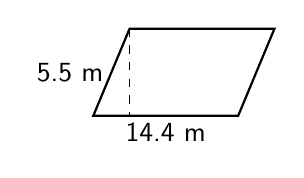
\begin{tikzpicture}[x=0.23cm,y=0.23cm,baseline=(current bounding box.center)]
  \coordinate (A) at (0,0);
  \coordinate (B) at (8,0);
  \coordinate (C) at (10,4.8);
  \coordinate (D) at (2,4.8);
  \draw[thick] (A)--(B)--(C)--(D)--cycle;
  \draw[dashed] (D)--(2,0);
  \node at (4,-0.9) {14.4 m};
  \node at (1.1,2.4) [left] {5.5 m};
\end{tikzpicture}
\task Find the area.\\[0.4em]
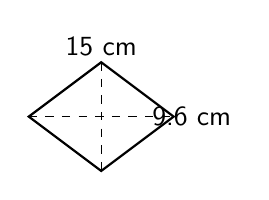
\begin{tikzpicture}[x=0.23cm,y=0.23cm,baseline=(current bounding box.center)]
  \coordinate (T) at (4,6);
  \coordinate (R) at (8,3);
  \coordinate (B) at (4,0);
  \coordinate (L) at (0,3);
  \draw[thick] (T)--(R)--(B)--(L)--cycle;
  \draw[dashed] (T)--(B);
  \draw[dashed] (L)--(R);
  \node at (4,6.9) {15 cm};
  \node at (9.0,3) {9.6 cm};
\end{tikzpicture}
\task A rectangle has area 96 cm\mbox{$^2$} and length 12 cm. Find the width.
\task A square has area 196 m\mbox{$^2$}. Find its perimeter.
\task A triangle has area 45 cm\mbox{$^2$} and height 6 cm. Find the base.
\task A parallelogram has the same base and height as a rectangle that is 11 cm by 4 cm. What is the area of the parallelogram?
\task A kite has area 84 cm\mbox{$^2$}. One diagonal is 14 cm. Find the other diagonal.
\task Which has greater area: a square of side 9 cm or a parallelogram with base 12 cm and height 7 cm? Show the difference.
\task A triangle and a kite both have area 54 cm\mbox{$^2$}. The triangle has base 12 cm. The kite has one diagonal 9 cm. Find the triangle's height and the kite's other diagonal.
\task A rectangle measures 18 cm by 7 cm. A triangle has the same area and base 14 cm. Find the triangle's height.
\task A student says, "A slanted side makes the area of a parallelogram bigger than a rectangle with the same base and perpendicular height." Explain why the student is wrong.
\task A square and a triangle both have area 64 cm\mbox{$^2$}. The square has side 8 cm. If the triangle has base 16 cm, find its height.
\task A kite has diagonals 20 cm and 12 cm. A triangle has the same area and base 15 cm. Find the triangle's height.
\task The area of a parallelogram is 72 m\mbox{$^2$}. If the base is tripled and the perpendicular height is halved, what is the new area?
\task Create two different rectangles with area 48 cm\mbox{$^2$} and explain how you know both are correct.
\end{tasks}

\end{document}
